\pgfdeclarelayer{background}
\pgfsetlayers{background,main}

\def\scale{0.85}
\def\upperlist{{(0, 8)/a}, {(1.5, 8)/b}, {(1, 6)/c}, {(2.5, 6)/d}}
\def\lowerlist{{(4.5, 3)/e}, {(7, 3)/f}, {(3, 1)/g}, {(6, 1)/h}}
\def\uppercon{a/b, a/c, c/b, c/d, b/d}
\def\lowercon{e/f, e/g, e/h, g/h, f/h}

\colorlet{circle edge}{black!50}

\tikzset{
  outline/.style={draw=circle edge, thick}
  filled/.style={draw=circle edge, thick}
  }

\tikzstyle{vertex}=[circle,fill=black!25,minimum size=10pt,inner sep=0pt]
\tikzstyle{invis-vertex}=[circle,fill=white!100,minimum size=0pt, inner sep=0pt]

\tikzstyle{edge} = [draw,thick,-]
\tikzstyle{weight} = [font=\small]

\tikzstyle{network_1} = [draw,line width=5pt,-,gray!50]
\tikzstyle{network_2} = [draw,line width=8pt,-,gray!80]
\tikzstyle{ignored edge} = [draw,line width=5pt,-,black!20]

% The connected network
\subfloat[]{\label{fig:network_part1}
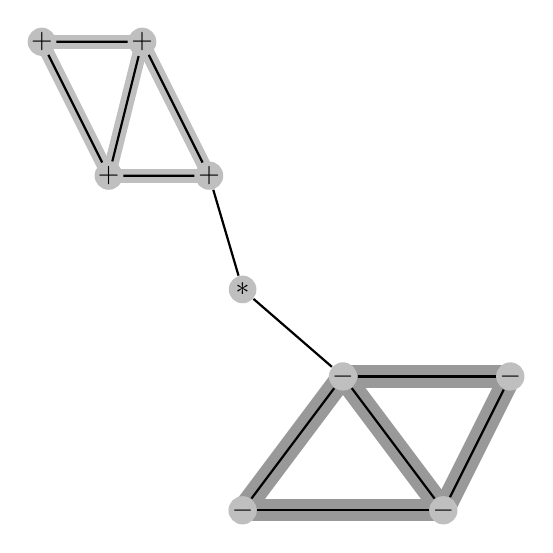
\begin{tikzpicture}[scale=\scale]
  % First we draw the vertices
  \foreach \pos/\name in \upperlist {
    \node[invis-vertex] (\name-) at \pos {};
    \node[vertex] (\name) at \pos {$+$};
  }   
   
  \foreach \pos/\name in \lowerlist {
    \node[invis-vertex] (\name-) at \pos {};
    \node[vertex] (\name) at \pos {$-$};
  }

  \node[vertex] (*) at (3, 4.3) {$*$};

  % Connect vertices with edges
  \foreach \source/ \dest in \uppercon
    \path[edge] (\source) -- (\dest);

  \foreach \source/ \dest in \lowercon
    \path[edge] (\source) -- (\dest);

  % Connect the lonely node
  \foreach \source/ \dest in {d/*, */e}
    \path[edge] (\source) -- (\dest);

  % Make the background
  \begin{pgfonlayer}{background}
    \foreach \source/\dest in \uppercon
      \path[network_1] (\source-) -- (\dest-);
      
    \foreach \source/ \dest in \lowercon
      \path[network_2] (\source-) -- (\dest-);
  \end{pgfonlayer}
\end{tikzpicture}}
% The unconnected network
\subfloat[]{\label{fig:network_part2}
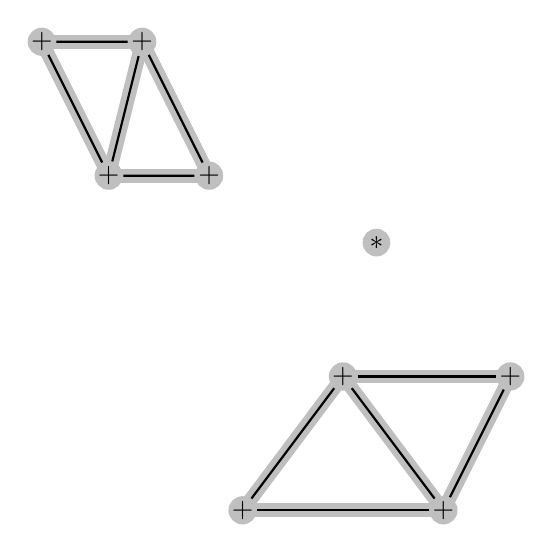
\begin{tikzpicture}[scale=\scale]
  %  First we draw the vertices
  \foreach \pos/\name in \upperlist {  
    \node[invis-vertex] (\name-) at \pos {};
    \node[vertex] (\name) at \pos {$+$};
  }   
   
  \foreach \pos/\name in \lowerlist {
    \node[invis-vertex] (\name-) at \pos {};
    \node[vertex] (\name) at \pos {$+$};
  }

  \node[vertex] (*) at (5, 5) {$*$};

  % Connect vertices with edges
  \foreach \source/ \dest in \uppercon
    \path[edge] (\source) -- (\dest);

  % Connect vertices with edges
  \foreach \source/ \dest in \lowercon
    \path[edge] (\source) -- (\dest);
    
  \begin{pgfonlayer}{background}
    \foreach \source/ \dest in \uppercon
      \path[network_1] (\source-) -- (\dest-);

    \foreach \source/ \dest in \lowercon
      \path[network_1] (\source-) -- (\dest-);
  \end{pgfonlayer}
\end{tikzpicture}}
